\documentclass{article}

\usepackage{fancyhdr}
\usepackage{extramarks}
\usepackage{amsmath}
\usepackage{amsthm}
\usepackage{amsfonts}
\usepackage{tikz}
\usepackage[american]{circuitikz} 
\usepackage[plain]{algorithm}
\usepackage{algpseudocode}
\usepackage{graphicx}
\usepackage{pgfplots}
\usepackage{subcaption}
\pgfplotsset{compat=1.18}

\usetikzlibrary{automata,positioning}

%
% Basic Document Settings
%

\topmargin=-0.45in
\evensidemargin=0in
\oddsidemargin=0in
\textwidth=6.5in
\textheight=9.0in
\headsep=0.25in

\linespread{1.1}

\pagestyle{fancy}
\lhead{Yousef Alaa Awad}
\chead{\hmwkClass\: \hmwkTitle}
\rhead{\firstxmark}
\lfoot{\lastxmark}
\cfoot{\thepage}

\renewcommand\headrulewidth{0.4pt}
\renewcommand\footrulewidth{0.4pt}

\setlength\parindent{0pt}

%
% Create Problem Sections
%

\setcounter{secnumdepth}{0}
\newcounter{partCounter}
\newcounter{homeworkProblemCounter}
\setcounter{homeworkProblemCounter}{1}

\newcommand{\hmwkTitle}{Homework\ \#4}
\newcommand{\hmwkDueDate}{March 2, 2026}
\newcommand{\hmwkClass}{Electronics 1}

%
% Title Page
%

\title{
    \vspace{2in}
    \textmd{\textbf{\hmwkClass:\ \hmwkTitle}}\\
    \normalsize\vspace{0.1in}
    \vspace{3in}
}

\author{Yousef Alaa Awad}

% Problems start here
\begin{document}

\maketitle
\pagebreak

\section{3.26}

\begin{figure}[h!]
    \centering
    \begin{circuitikz}[scale=1.0, transform shape]
        \draw (0,4) node[vcc]{$V_{DD} = 10\text{ V}$} -- (0,3);
        \draw (0,3) -- (-2.5,3) to[R, l=$R_1$, a=$32\text{ k}\Omega$] (-2.5,0) to[R, l=$R_2$, a=$18\text{ k}\Omega$] (-2.5,-3) node[ground]{};
        \draw (0,3) -- (2,3) to[R, l=$R_D$, a=$4\text{ k}\Omega$] (2,1);
        \draw (2,0) node[nmos](M1){};
        \draw (-2.5,0) -- (M1.G);
        \draw (2,1) -- (M1.D);
        \draw (M1.S) -- (2,-1) to[R, l=$R_S$, a=$2\text{ k}\Omega$] (2,-3) node[ground]{};
    \end{circuitikz}
    \caption{Circuit for Problem 3.26}
\end{figure}

Given parameters for the NMOS: $V_{TN} = 0.8\text{ V}$, $K_n = 0.5\text{ mA/V}^2$.
Using the voltage divider to find the gate voltage $V_G$:
$$ V_G = V_{DD} \left( \frac{R_2}{R_1 + R_2} \right) = 10 \left( \frac{18}{32 + 18} \right) = 3.6\text{ V} $$

The source voltage $V_S$ is found by:
$$ V_S = I_D R_S = I_D(2\text{ k}\Omega) = 2I_D $$
Thus, the gate-to-source voltage $V_{GS}$ is:
$$ V_{GS} = V_G - V_S = 3.6 - 2I_D $$

Assuming the transistor is in the saturation region:
$$ I_D = K_n (V_{GS} - V_{TN})^2 $$
$$ I_D = 0.5 (3.6 - 2I_D - 0.8)^2 = 0.5 (2.8 - 2I_D)^2 $$
$$ I_D = 0.5 (7.84 - 11.2I_D + 4I_D^2) = 3.92 - 5.6I_D + 2I_D^2 $$

Rearranging into a standard quadratic equation:
$$ 2I_D^2 - 6.6I_D + 3.92 = 0 $$
Solving for $I_D$:
$$ I_D = \frac{6.6 \pm \sqrt{43.56 - 4(2)(3.92)}}{4} = \frac{6.6 \pm \sqrt{12.2}}{4} $$
The two possible solutions are $I_D = 2.52\text{ mA}$ and $I_D = 0.777\text{ mA}$.
If $I_D = 2.52\text{ mA}$, then $V_{GS} = 3.6 - 2(2.52) = -1.44\text{ V}$, which implies the transistor is off ($V_{GS} < V_{TN}$). Therefore, this solution is invalid.
Using the valid solution $I_D = 0.777\text{ mA}$:
$$ V_{GS} = 3.6 - 2(0.777) = 2.046\text{ V} $$

Now calculate $V_{DS}$ to verify the saturation region:
$$ V_{DS} = V_{DD} - I_D(R_D + R_S) = 10 - 0.777(4 + 2) = 10 - 4.662 = 5.338\text{ V} $$
Checking saturation condition:
$$ V_{DS} \geq V_{GS} - V_{TN} \implies 5.338\text{ V} \geq 2.046\text{ V} - 0.8\text{ V} = 1.246\text{ V} $$
The assumption holds. The Q-point values are:
**$V_{GS} = 2.046\text{ V}$, $I_D = 0.777\text{ mA}$, $V_{DS} = 5.338\text{ V}$**.

\pagebreak
\section{3.31}

\begin{figure}[h!]
    \centering
    \begin{circuitikz}[scale=1.0, transform shape]
        \draw (0,3) node[vcc]{$+5\text{ V}$} to[I, l=$I_Q$, a=$0.4\text{ mA}$] (0,1);
        \draw (0,0) node[pmos](M1){};
        \draw (0,1) -- (M1.S);
        \draw (M1.S) to[short, *-o] (1.5,0.78) node[right]{$V_S$};
        \draw (M1.D) to[R, l=$R_D$, a=$5\text{ k}\Omega$] (0,-3) node[vee]{$-5\text{ V}$};
        \draw (M1.G) -- (-2,0) to[R, l=$R_G$, a=$50\text{ k}\Omega$] (-2,-2) node[ground]{};
    \end{circuitikz}
    \caption{Circuit for Problem 3.31}
\end{figure}

Given parameters for the PMOS: $V_{TP} = -0.8\text{ V}$, $K_p = 200\text{ }\mu\text{A/V}^2 = 0.2\text{ mA/V}^2$, and $I_Q = 0.4\text{ mA}$.
Since the gate is tied to ground through $R_G$ and no DC gate current flows ($I_G = 0$), the gate voltage is $V_G = 0\text{ V}$.
The drain current $I_D$ is set directly by the current source $I_Q$:
$$ I_D = 0.4\text{ mA} $$

Assume the PMOS is in saturation:
$$ I_D = K_p(V_{SG} + V_{TP})^2 \implies 0.4 = 0.2(V_{SG} - 0.8)^2 $$
$$ (V_{SG} - 0.8)^2 = 2 \implies V_{SG} - 0.8 = \sqrt{2} \approx 1.414\text{ V} $$
$$ V_{SG} = 2.214\text{ V} $$

Since $V_G = 0\text{ V}$ and $V_{SG} = V_S - V_G$:
$$ V_S = 2.214\text{ V} $$

To find $V_{SD}$, we first determine the drain voltage $V_D$:
$$ V_D = -5 + I_D R_D = -5 + (0.4\text{ mA})(5\text{ k}\Omega) = -5 + 2 = -3\text{ V} $$
Now we calculate $V_{SD}$:
$$ V_{SD} = V_S - V_D = 2.214 - (-3) = 5.214\text{ V} $$

Checking the saturation condition ($V_{SD} \geq V_{SG} + V_{TP}$):
$$ 5.214\text{ V} \geq 2.214\text{ V} - 0.8\text{ V} = 1.414\text{ V} $$
The assumption holds.
**$V_S = 2.214\text{ V}$ and $V_{SD} = 5.214\text{ V}$**.

\pagebreak
\section{3.35}

\begin{figure}[h!]
    \centering
    \begin{circuitikz}[scale=1.0, transform shape]
        \draw (0,4) node[vcc]{$+5\text{ V}$} -- (0,3);
        \draw (0,3) -- (-2.5,3) to[R, l=$R_1$, a=$14\text{ k}\Omega$] (-2.5,0) to[R, l=$R_2$, a=$6\text{ k}\Omega$] (-2.5,-3);
        \draw (0,3) -- (2,3) to[R, l=$R_D$, a=$1.2\text{ k}\Omega$] (2,1);
        \draw (2,0) node[nmos](M1){};
        \draw (-2.5,0) -- (M1.G);
        \draw (2,1) -- (M1.D);
        \draw (M1.S) -- (2,-1) to[R, l=$R_S$, a=$0.5\text{ k}\Omega$] (2,-3);
        \draw (-2.5,-3) -- (2,-3); % Connecting the bottom rail
        \draw (0,-3) node[vee]{$-5\text{ V}$}; % The -5V node in the middle
    \end{circuitikz}
    \caption{Circuit for Problem 3.35}
\end{figure}

Given parameters: $V_{TN} = 0.4\text{ V}$, $k'_n = 120\text{ }\mu\text{A/V}^2 = 0.12\text{ mA/V}^2$, $W/L = 25$.
First, calculate $K_n$:
$$ K_n = \frac{1}{2} k'_n \left(\frac{W}{L}\right) = \frac{1}{2}(0.12)(25) = 1.5\text{ mA/V}^2 $$

Calculate the gate voltage $V_G$ via the voltage divider from the $10\text{ V}$ total supply ($+5\text{ V}$ to $-5\text{ V}$):
$$ V_G = -5 + \left(\frac{6}{14 + 6}\right) \cdot (10) = -5 + 3 = -2\text{ V} $$

The source voltage is given by:
$$ V_S = -5 + I_D R_S = -5 + 0.5I_D $$
$$ V_{GS} = V_G - V_S = -2 - (-5 + 0.5I_D) = 3 - 0.5I_D $$

Assuming saturation:
$$ I_D = K_n(V_{GS} - V_{TN})^2 = 1.5(3 - 0.5I_D - 0.4)^2 = 1.5(2.6 - 0.5I_D)^2 $$
$$ I_D = 1.5(6.76 - 2.6I_D + 0.25I_D^2) = 10.14 - 3.9I_D + 0.375I_D^2 $$
$$ 0.375I_D^2 - 4.9I_D + 10.14 = 0 $$

Solving for $I_D$:
$$ I_D = \frac{4.9 \pm \sqrt{24.01 - 4(0.375)(10.14)}}{0.75} = \frac{4.9 \pm \sqrt{8.8}}{0.75} $$
$I_D = 10.49\text{ mA}$ or $I_D = 2.578\text{ mA}$.
If $I_D = 10.49\text{ mA}$, then $V_S = -5 + 0.5(10.49) = 0.245\text{ V}$, and $V_{GS} = -2 - 0.245 = -2.245\text{ V}$ (Invalid, off).
Using $I_D = 2.578\text{ mA}$:
$$ V_S = -5 + 0.5(2.578) = -3.711\text{ V} \implies V_{GS} = -2 - (-3.711) = 1.711\text{ V} $$

Now calculate $V_{DS}$:
$$ V_{DS} = V_D - V_S = (5 - I_D R_D) - (-3.711) = (5 - 2.578 \cdot 1.2) + 3.711 = 1.906 + 3.711 = 5.617\text{ V} $$
Saturation verified ($5.617 > 1.711 - 0.4$).
**$V_{GS} = 1.711\text{ V}$, $I_D = 2.578\text{ mA}$, $V_{DS} = 5.617\text{ V}$**.

\begin{figure}[h!]
    \centering
    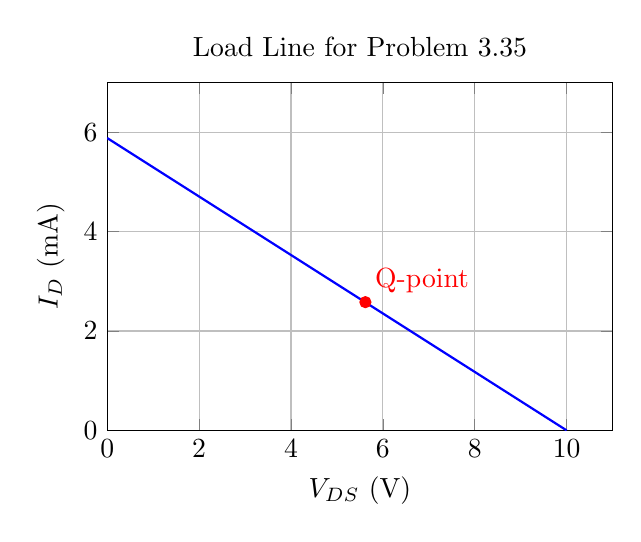
\begin{tikzpicture}
        \begin{axis}[
            title={Load Line for Problem 3.35},
            xlabel={$V_{DS}$ (V)},
            ylabel={$I_D$ (mA)},
            xmin=0, xmax=11,
            ymin=0, ymax=7,
            grid=both,
            width=8cm,
            height=6cm
        ]
        \addplot [blue, thick, domain=0:10] { (10 - x)/1.7 };
        \addplot [red, only marks, mark=*] coordinates { (5.62, 2.58) } node[above right] {Q-point};
        \end{axis}
    \end{tikzpicture}
    \caption{DC Load Line and Q-Point}
\end{figure}

\pagebreak
\section{3.43}

\begin{figure}[h!]
    \centering
    \begin{circuitikz}[scale=1.0, transform shape]
        \draw (0,3) node[vcc]{$+5\text{ V}$} to[R, l=$R_1$] (0,0);
        \draw (0,0) node[circ]{} to[R, l=$R_2$] (0,-3) node[vee]{$-5\text{ V}$};
        \draw (2,0) node[pmos](M1){};
        \draw (0,0) -- (M1.G);
        \draw (M1.S) -- (2,2) -- (3,2) node[ground]{};
        \draw (M1.D) to[R, l=$R_D$] (2,-3) node[vee]{$-10\text{ V}$};
        \draw (0,0) -- (-2,0);
        \draw[dashed] (-1,0.8) -- (-1,-0.8);
        \draw[-latex] (-2,0.4) node[above]{$R_{\text{in}}$} -- (-1.1,0.4);
    \end{circuitikz}
    \caption{Circuit for Problem 3.43}
\end{figure}

Given PMOS parameters: $V_{TP} = -1.75\text{ V}$, $K_p = 3\text{ mA/V}^2$.
Design requirements: $I_D = 5\text{ mA}$, $V_{SD} = 6\text{ V}$, and $R_{in} = 80\text{ k}\Omega$.

The source is tied to ground, so $V_S = 0\text{ V}$.
For $V_{SD} = 6\text{ V}$:
$$ V_{SD} = V_S - V_D \implies 6 = 0 - V_D \implies V_D = -6\text{ V} $$
The drain current flows through $R_D$ to the $-10\text{ V}$ supply:
$$ V_D = -10 + I_D R_D \implies -6 = -10 + (5\text{ mA})R_D \implies R_D = \frac{4}{5} = 0.8\text{ k}\Omega = 800\text{ }\Omega $$

Assume PMOS is in saturation to find the required $V_{SG}$:
$$ I_D = K_p(V_{SG} + V_{TP})^2 \implies 5 = 3(V_{SG} - 1.75)^2 $$
$$ (V_{SG} - 1.75)^2 = 1.667 \implies V_{SG} - 1.75 \approx 1.291\text{ V} \implies V_{SG} = 3.041\text{ V} $$
Since $V_S = 0\text{ V}$, the gate voltage must be $V_G = -3.041\text{ V}$.

The gate voltage is established by the $R_1$ and $R_2$ voltage divider:
$$ V_G = -5 + \left(\frac{R_2}{R_1 + R_2}\right) \cdot (10) $$
Let $x = \frac{R_2}{R_1 + R_2}$. Then:
$$ -3.041 = -5 + 10x \implies 10x = 1.959 \implies x = 0.1959 $$

The input resistance is the parallel combination of $R_1$ and $R_2$:
$$ R_{in} = R_1 \parallel R_2 = 80\text{ k}\Omega $$
Using the relationship $R_{in} = x \cdot R_1$:
$$ R_1 = \frac{R_{in}}{x} = \frac{80\text{ k}\Omega}{0.1959} \approx 408.37\text{ k}\Omega $$
Using the parallel combination to find $R_2$:
$$ 80 = \frac{408.37 \cdot R_2}{408.37 + R_2} \implies R_2 = \frac{80 \cdot 408.37}{408.37 - 80} = \frac{32669.6}{328.37} \approx 99.49\text{ k}\Omega $$

**Design values:** $R_D = 0.8\text{ k}\Omega$, $R_1 = 408.37\text{ k}\Omega$, $R_2 = 99.49\text{ k}\Omega$.

\end{document}
